\documentclass[11pt,a4paper]{article}

% ===================== PACKAGES =====================
\usepackage[T1]{fontenc}
\usepackage[utf8]{inputenc}
\usepackage[a4paper,margin=2.4cm]{geometry}
\usepackage{amssymb}
\usepackage[table]{xcolor}
\usepackage{booktabs}
\usepackage{longtable}
\usepackage{array}
\usepackage{tabularx}
\usepackage{enumitem}
\usepackage{titlesec}
\usepackage{graphicx}
\usepackage{float}
\usepackage{caption}
\usepackage{fancyhdr}
\usepackage[hidelinks]{hyperref}

% ===================== STYLING =====================
\definecolor{antamblue}{RGB}{0,51,102}
\definecolor{antamgold}{RGB}{197,148,40}
\definecolor{softgray}{RGB}{242,244,247}
\definecolor{darkgray}{RGB}{90,90,90}

\titleformat{\section}{\color{antamblue}\Large\bfseries}{\thesection.}{0.6em}{}
\titleformat{\subsection}{\color{antamblue}\large\bfseries}{\thesubsection}{0.6em}{}
\titlespacing*{\section}{0pt}{1.3em}{0.6em}

\captionsetup{font=small,labelfont={bf,color=antamblue},labelsep=period}
\setlist[itemize]{leftmargin=1.4em,topsep=2pt,itemsep=1pt}
\setlist[enumerate]{leftmargin=1.6em,topsep=2pt,itemsep=1pt}
\newcolumntype{Y}{>{\raggedright\arraybackslash}X}
\newcolumntype{C}{>{\centering\arraybackslash}X}
\renewcommand{\arraystretch}{1.25}

% Callout box
\newcommand{\callout}[2]{%
  \begin{center}\colorbox{softgray}{\parbox{0.96\linewidth}{%
  \vspace{2pt}\textbf{\color{antamblue}#1}\\[2pt]#2\vspace{2pt}}}\end{center}}

\pagestyle{fancy}\fancyhf{}
\renewcommand{\headrulewidth}{0.4pt}
\fancyhead[L]{\small\color{darkgray}NickelScope --- ANTAM Hackathon 2026}
\fancyhead[R]{\small\color{darkgray}Tema: Eksplorasi}
\fancyfoot[C]{\small\color{darkgray}\thepage}

\hypersetup{
  pdftitle={NickelScope - Proposal},
  pdfauthor={Tim NickelScope},
  colorlinks=true, linkcolor=antamblue, urlcolor=antamgold, citecolor=antamblue
}

% ===================== TITLE =====================
\begin{document}
\thispagestyle{empty}

\begin{center}
{\color{antamgold}\rule{\linewidth}{1.5pt}}\\[0.8em]
{\color{antamblue}\Huge\bfseries NickelScope}\\[0.5em]
{\color{antamblue}\large AI--GIS Prospectivity Mapping untuk Eksplorasi\\
Nikel Laterit Berbasis Penginderaan Jauh}\\[0.8em]
{\color{antamgold}\rule{\linewidth}{1.5pt}}\\[1.2em]

\begin{tabularx}{0.85\linewidth}{@{}>{\bfseries\color{antamblue}}r X@{}}
Lomba    & ANTAM Hackathon 2026 --- Young Mining Innovators \\
Tema     & 1. Eksplorasi \\
Komoditas & Nikel Laterit \\
Studi Kasus & Sabuk Pomalaa--Kolaka, Sulawesi Tenggara \\
Tim      & \textit{(nama tim \& anggota)} \\
Tanggal  & \today \\
\end{tabularx}
\end{center}

\vspace{0.6em}
\callout{Ringkasan Eksekutif}{%
NickelScope adalah sistem AI--GIS yang memetakan \textbf{probabilitas keterdapatan
nikel laterit} dengan memfusikan citra satelit, model elevasi digital, dan peta
geologi resmi, lalu \textbf{membatasi prediksi pada batuan induk ultramafik
(host-rock constraint)}. Output utamanya adalah \textbf{peta target bor prioritas}
yang tervalidasi geologis, sehingga eksplorasi menjadi lebih hemat biaya, lebih
cepat, dan lebih bertanggung jawab terhadap lingkungan. Seluruh pipeline dibangun
\textbf{100\% dari data publik dan perangkat open-source}, dan telah menghasilkan
purwarupa peta prospektivitas dengan \textbf{Spatial CV AUC 0,986} yang tervalidasi
secara geologis.}

\vspace{0.4em}
{\small\itshape Catatan integritas data: studi ini menggunakan data publik
(Sentinel-2, SRTM, GeoMap ESDM), \textbf{bukan} data internal ANTAM.}

\tableofcontents
\vspace{0.5em}\hrule
\newpage

% ===================================================================
\section{Latar Belakang \& Pernyataan Masalah}

Eksplorasi nikel laterit konvensional sangat bergantung pada pengeboran intensif
yang \textbf{mahal, lambat, dan kerap ``buta''} --- banyak lubang bor jatuh pada
area non-prospektif. Padahal nikel adalah komoditas andalan PT ANTAM dan tulang
punggung rantai nilai baterai kendaraan listrik nasional.

\begin{itemize}
  \item \textbf{Biaya.} Satu titik bor eksplorasi dapat menelan puluhan hingga
  ratusan juta rupiah; pengeboran tak terarah berarti pemborosan besar.
  \item \textbf{Waktu.} Siklus eksplorasi yang panjang memperlambat konversi
  sumber daya menjadi cadangan.
  \item \textbf{Risiko \& ESG.} Pengeboran di area sensitif (lereng curam, sungai,
  kawasan lindung) menambah jejak lingkungan dan risiko K3.
\end{itemize}

\callout{Pernyataan Masalah}{%
Bagaimana mengarahkan kegiatan eksplorasi dan pengeboran nikel laterit secara
lebih cerdas, hemat, dan bertanggung jawab menggunakan data yang tersedia secara
publik --- \textit{sebelum} alat berat masuk ke lapangan?}

% ===================================================================
\section{Tujuan \& Cakupan Studi Kasus}

\textbf{Tujuan.} Membangun sistem AI--GIS yang menghasilkan peta probabilitas
prospektivitas nikel laterit dan daftar target bor prioritas yang
tervalidasi geologis, dengan metodologi yang jujur dan dapat direproduksi.

\textbf{Lokasi (terkunci).} Sabuk \textbf{Pomalaa--Kolaka}, Sulawesi Tenggara ---
bagian dari \textit{East Sulawesi Ophiolite Belt} dan salah satu aset nikel
utama ANTAM.
\begin{itemize}
  \item \textbf{AOI bounding box:} Lat $-4{,}35^\circ$ s/d $-3{,}95^\circ$;
  Lon $121{,}50^\circ$ s/d $121{,}75^\circ$ ($\sim$28 km $\times$ 44 km).
  \item Mencakup distrik tambang Pomalaa (Tambang Utara \& Selatan) hingga selatan Kolaka.
\end{itemize}

\textbf{Batas asumsi.} Model berbasis \textit{proxy} permukaan (penginderaan jauh
+ topografi + geologi), \textbf{bukan pengganti pengeboran}. Output adalah
\textit{prioritisasi}, bukan kepastian keterdapatan.

\begin{figure}[H]\centering
  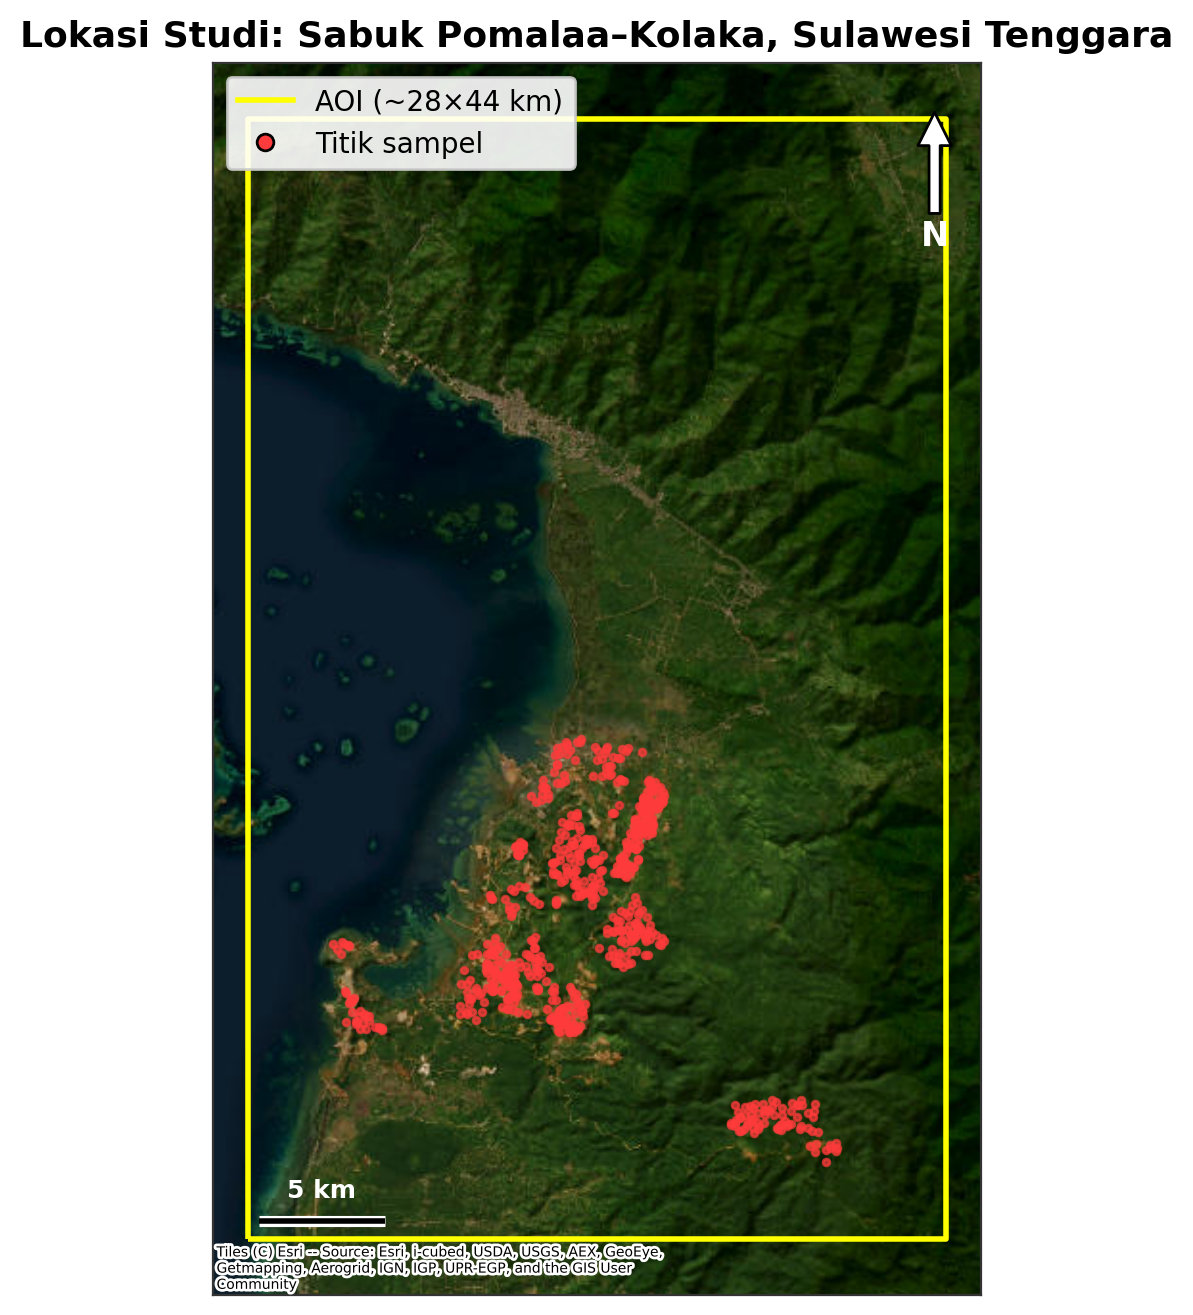
\includegraphics[width=0.82\linewidth]{figures/fig1_lokasi.png}
  \caption{Lokasi area studi (AOI) Sabuk Pomalaa--Kolaka, Sulawesi Tenggara.}
  \label{fig:lokasi}
\end{figure}

% ===================================================================
\section{Data \& Metode}

\subsection{Sumber Data (publik \& legal)}

\begin{tabularx}{\linewidth}{@{}>{\bfseries}l Y l@{}}
\toprule
Data & Sumber & Peran \\
\midrule
Sentinel-2 (10--20 m) & Copernicus / Google Earth Engine & Indeks besi, alterasi, vegetasi \\
DEM SRTM (30 m)       & USGS / Google Earth Engine        & Slope, elevasi, curvature, TWI \\
MERIT Hydro           & Flow accumulation                 & Komponen TWI (pelindian) \\
Peta Geologi 1:100k   & GeoMap --- Badan Geologi ESDM     & Host-rock ultramafik \\
Konsesi tambang (ref) & MOMI / Geoportal ESDM             & Acuan pelabelan \\
\bottomrule
\end{tabularx}

\subsection{Feature Engineering (keunggulan domain geologi tim)}

Delapan fitur dibangun dari pengetahuan genesis laterit:
\begin{itemize}
  \item \textbf{Spektral (Sentinel-2):} \textit{iron-oxide ratio} (B4/B2),
  \textit{ferrous}, \textit{clay ratio}, dan \textbf{NDVI} --- penanda
  tanah laterit kaya Fe-oksida dan tutupan vegetasi.
  \item \textbf{Topografi (DEM):} \textbf{elevasi}, \textbf{slope},
  \textbf{curvature}, dan \textbf{TWI} --- laterit terbentuk \& terawetkan
  pada permukaan landai-stabil; TWI mengontrol pelindian (\textit{leaching}) Ni.
\end{itemize}

\begin{figure}[H]\centering
  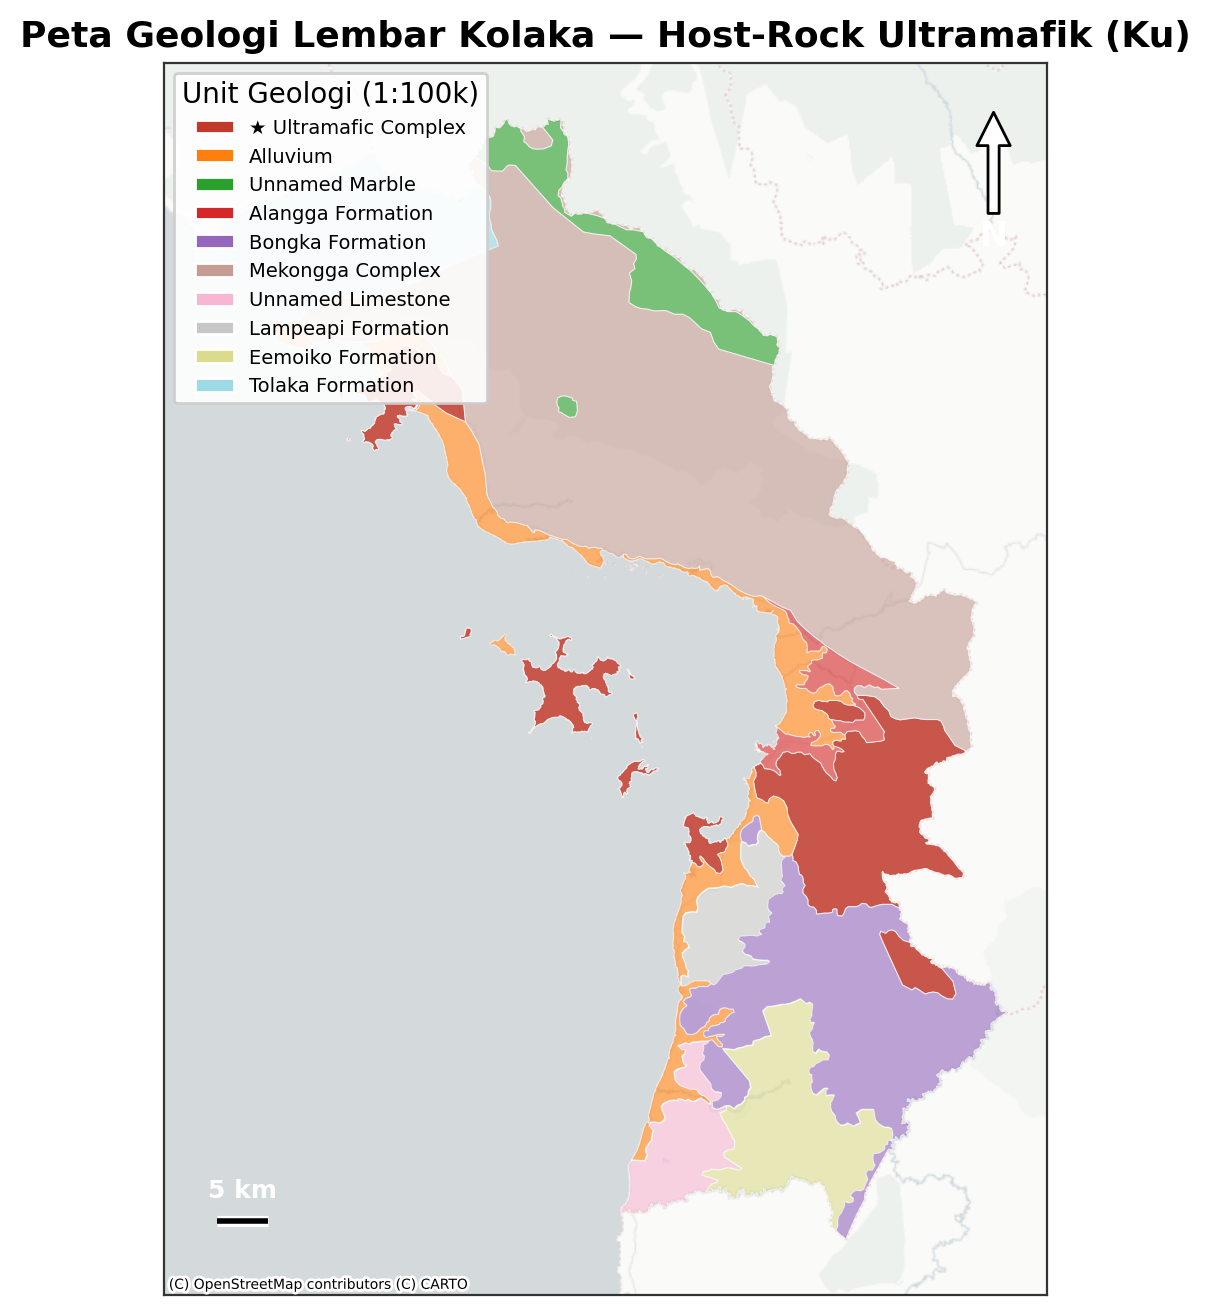
\includegraphics[width=0.49\linewidth]{figures/fig2_geologi.png}\hfill
  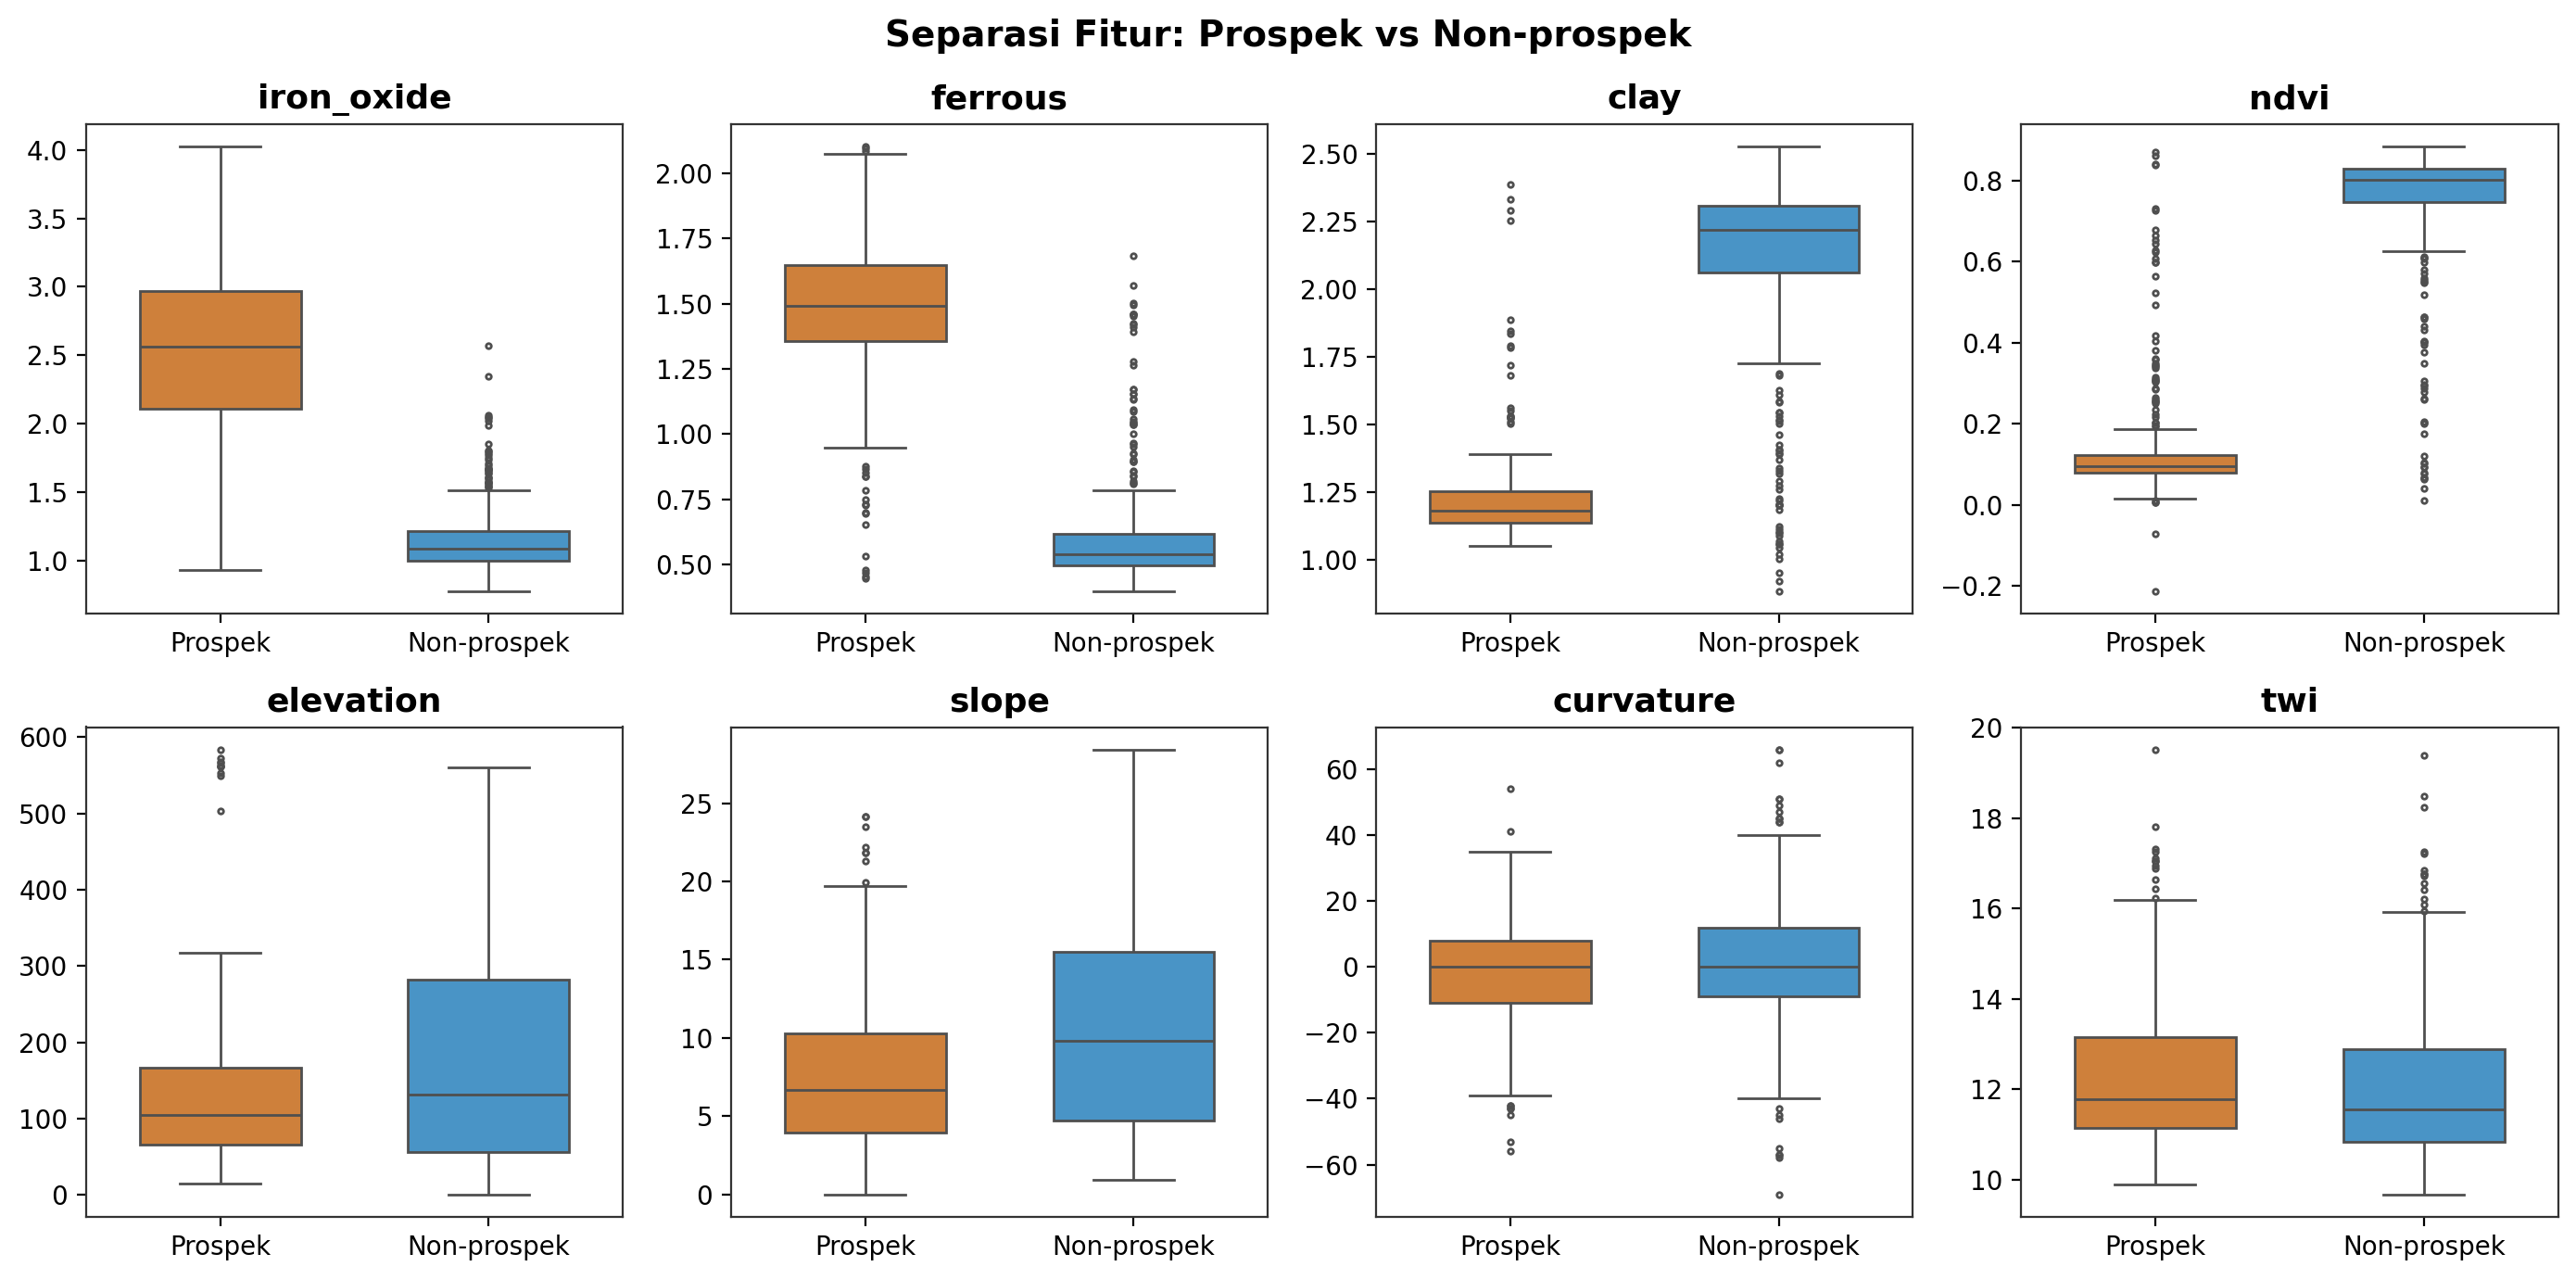
\includegraphics[width=0.49\linewidth]{figures/fig5_fitur_boxplot.png}
  \caption{Kiri: peta geologi resmi (unit ultramafik sebagai host-rock).
  Kanan: sebaran nilai fitur untuk titik prospektif vs non-prospektif.}
  \label{fig:geo_box}
\end{figure}

\subsection{Pemodelan \& Validasi}

\begin{enumerate}
  \item \textbf{Pelabelan.} Footprint laterit terbuka dideteksi dari Sentinel-2
  (indeks besi + NDVI), lalu di-\textit{sampling} menjadi 650 titik berlabel
  (positif/negatif).
  \item \textbf{Model.} Random Forest (utama) dan XGBoost (pembanding).
  \item \textbf{Validasi jujur.} \textbf{Spatial (block) cross-validation}
  --- bukan \textit{random split} --- agar autokorelasi spasial tidak
  menggelembungkan performa.
  \item \textbf{Host-rock constraint.} Prediksi divalidasi \& dibatasi dengan
  peta geologi resmi (lihat Bagian~\ref{sec:temuan}).
\end{enumerate}

% ===================================================================
\section{Temuan Kunci: Dari Model Menyesatkan ke Model Jujur}
\label{sec:temuan}

\textbf{Inilah inti metodologi NickelScope.} Model spektral naif menghasilkan
\textbf{Spatial AUC 0,988} yang terlihat luar biasa --- namun \textit{menyesatkan}.
Karena label positif diambil dari permukaan laterit \textit{tersingkap}, fitur
spektral mendominasi (besar) dan model sesungguhnya menjadi
\textbf{``detektor lahan terbuka''}, bukan prediktor prospektivitas sejati.

\textbf{Validasi silang dengan geologi resmi} (GeoMap 1:100k Kolaka, WGS84)
mengungkap kontaminasi label: hanya \textbf{42\%} (127/300) titik positif awal
benar-benar berada di dalam unit ultramafik; sisanya tersebar pada formasi
sedimen (molasse) dengan median jarak \textbf{1,3 km} dari host-rock.

\begin{figure}[H]\centering
  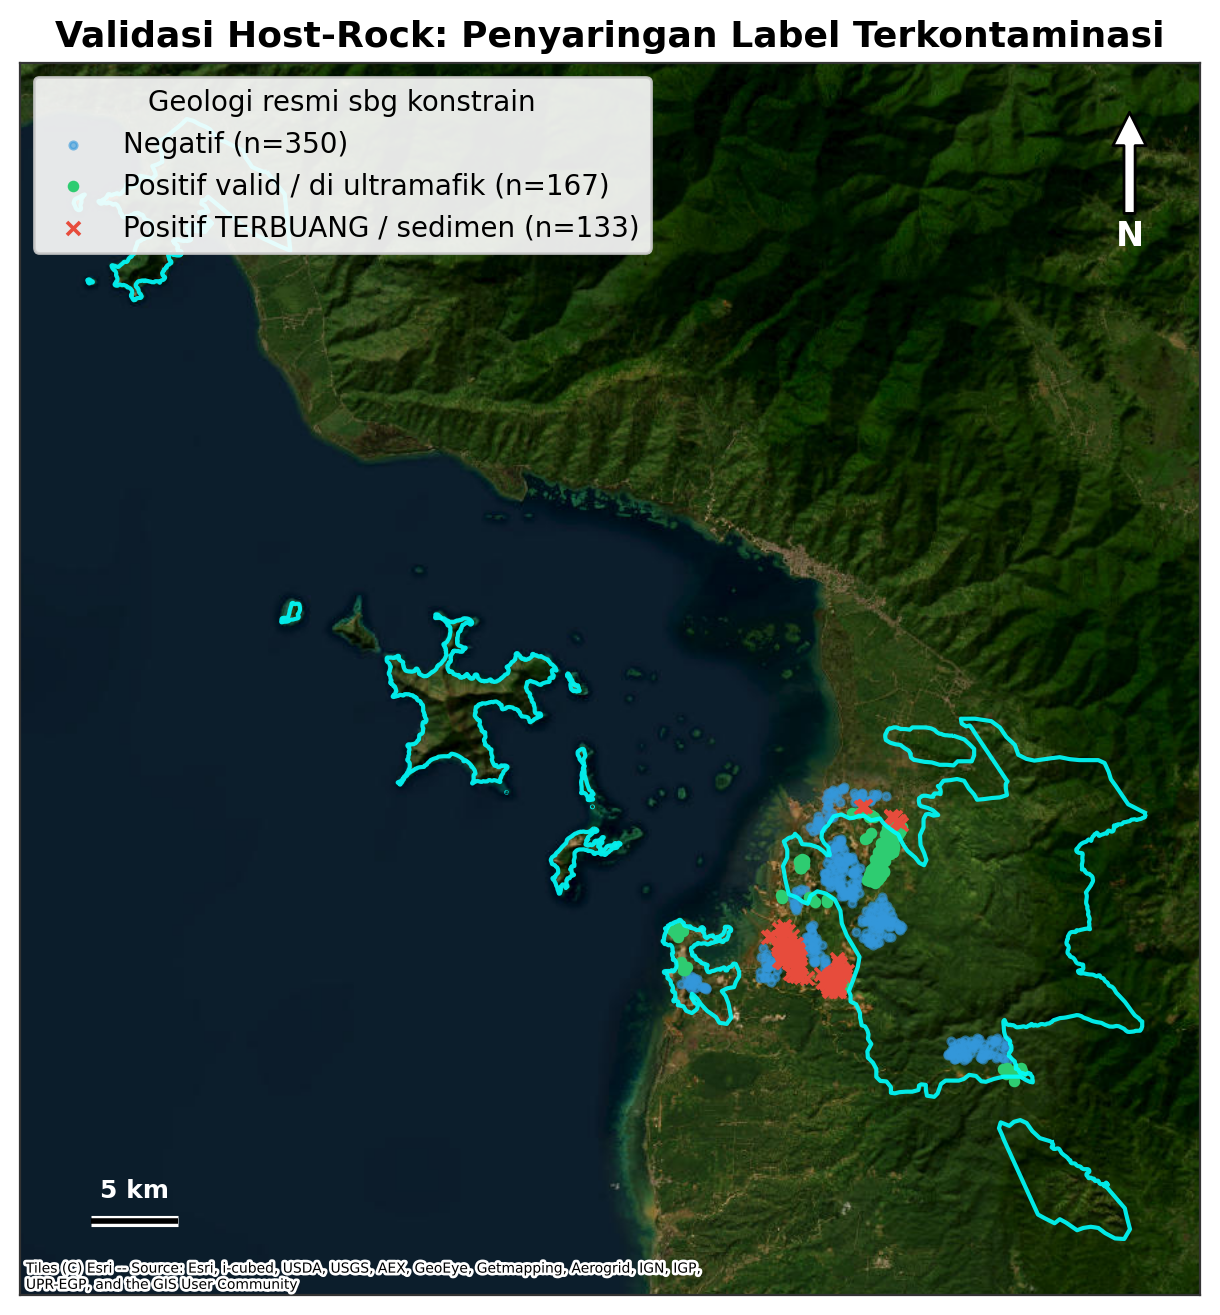
\includegraphics[width=0.49\linewidth]{figures/fig3_label_hostrock.png}\hfill
  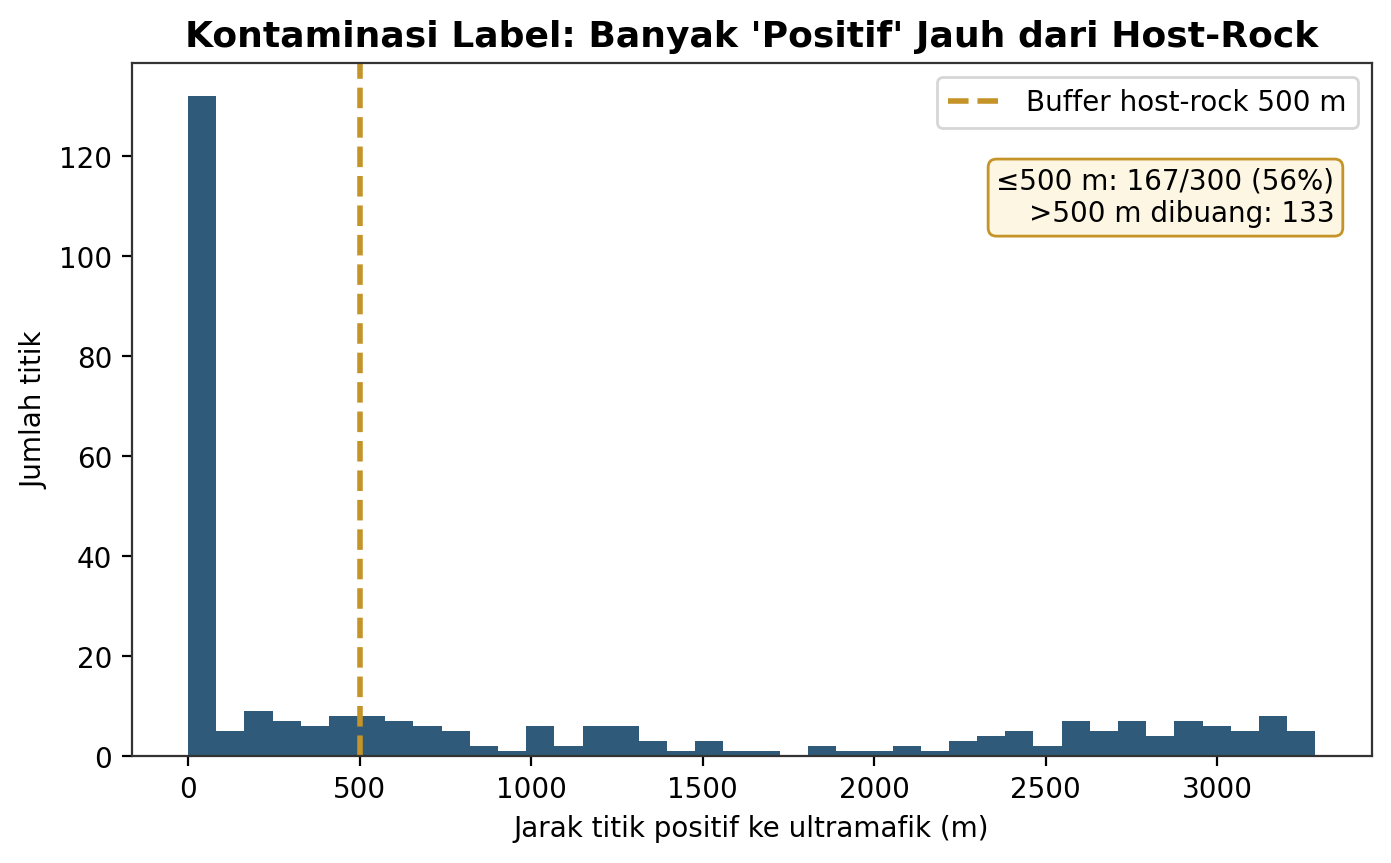
\includegraphics[width=0.49\linewidth]{figures/fig4_dist_hist.png}
  \caption{Kiri: penyaringan label terhadap host-rock ultramafik (titik valid vs
  terkontaminasi). Kanan: distribusi jarak titik positif ke unit ultramafik.}
  \label{fig:label}
\end{figure}

\textbf{Perbaikan.} Label disaring ke domain host-rock (ultramafik + buffer 500 m);
133 positif terkontaminasi dibuang, lalu model dilatih ulang. Hasilnya tetap kuat
\textbf{tanpa kehilangan akurasi} --- dan kini \textbf{valid secara geologis}.

\begin{table}[H]\centering\small
\begin{tabular}{@{}lcl@{}}
\toprule
\textbf{Model} & \textbf{Spatial CV AUC} & \textbf{Catatan} \\
\midrule
Naif (terkontaminasi) & 0,988 & Mendeteksi lahan terbuka --- circular \\
\rowcolor{softgray}\textbf{Host-Rock Constrained} & \textbf{0,986} & \textbf{Valid geologis} (133 FP dibuang) \\
\bottomrule
\end{tabular}
\caption{Perbandingan performa: angka tinggi yang jujur mengalahkan angka tinggi yang menyesatkan.}
\end{table}

\begin{figure}[H]\centering
  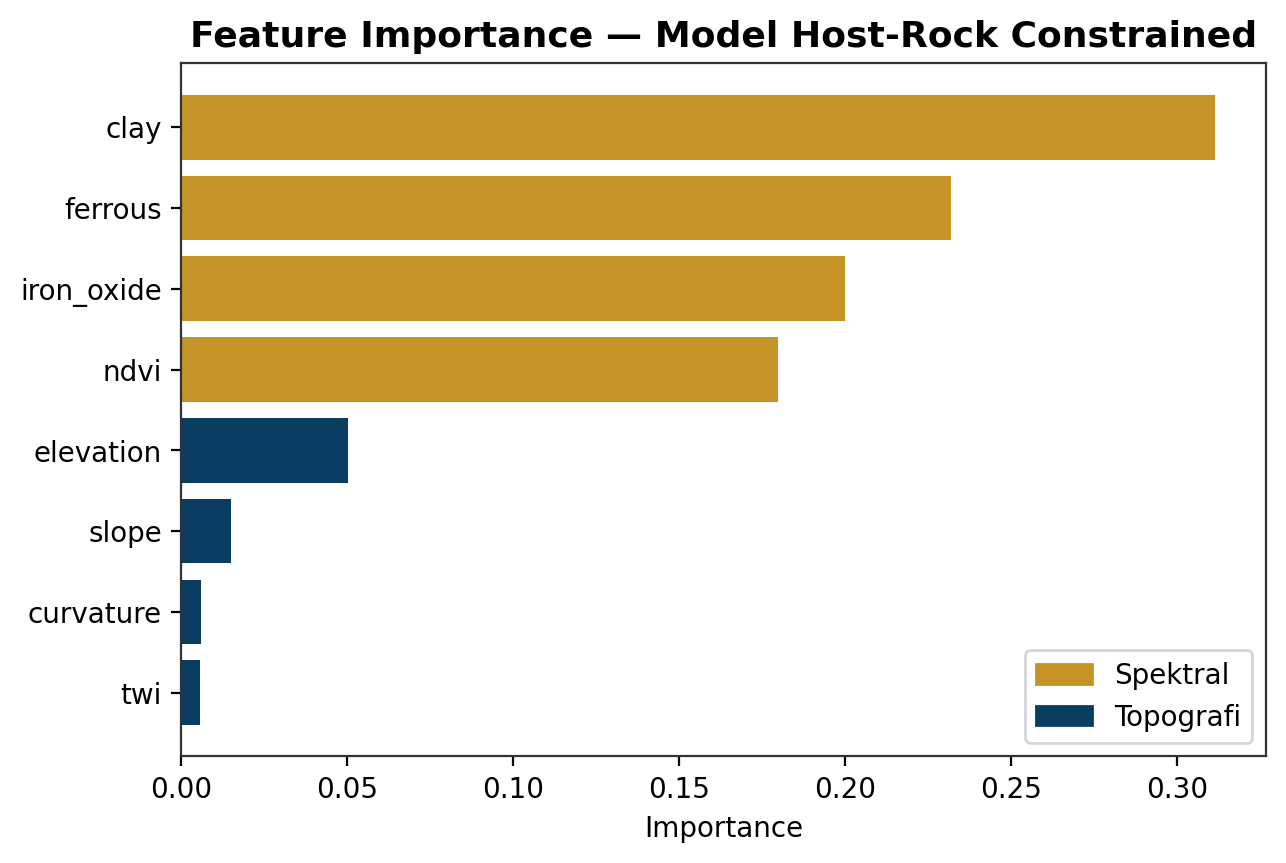
\includegraphics[width=0.32\linewidth]{figures/fig7_importance.png}\hfill
  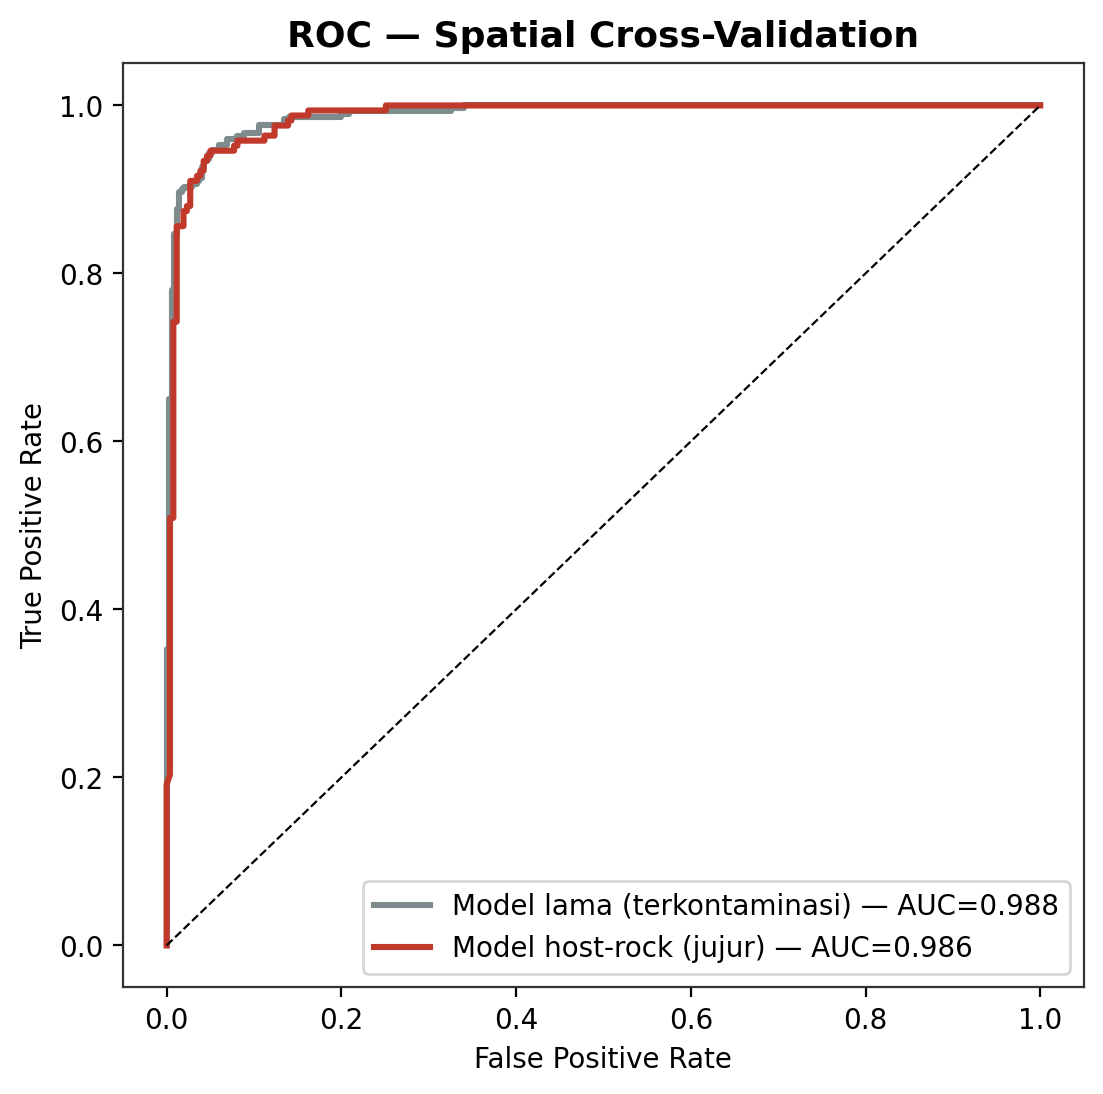
\includegraphics[width=0.32\linewidth]{figures/fig8_roc.png}\hfill
  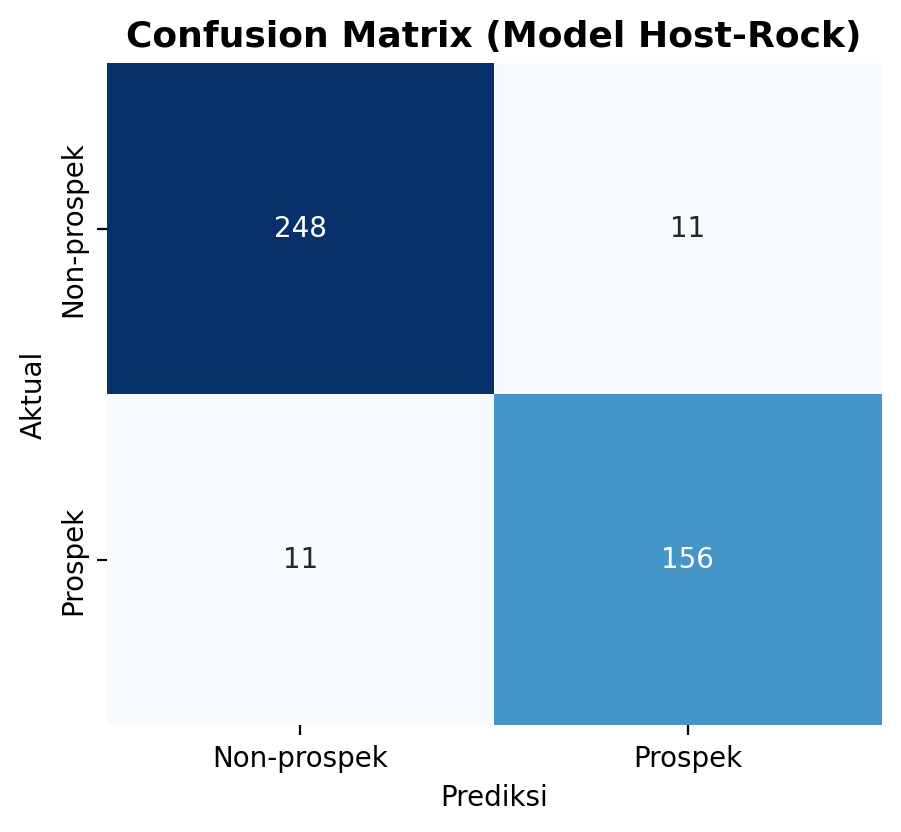
\includegraphics[width=0.32\linewidth]{figures/fig9_confusion.png}
  \caption{Kiri: kepentingan fitur model jujur. Tengah: kurva ROC spatial CV
  (naif vs jujur). Kanan: matriks konfusi model host-rock.}
  \label{fig:metrics}
\end{figure}

\callout{Mengapa ini keunggulan, bukan kelemahan}{%
Banyak solusi akan berhenti di AUC 0,988 dan menyebutnya ``akurat''. NickelScope
justru \textbf{mengaudit modelnya sendiri dengan geologi resmi}, mengakui
sirkularitas, dan memperbaikinya. Inilah praktik eksplorasi yang
bertanggung jawab --- keputusan bor yang didasari model yang jujur.}

% ===================================================================
\section{Hasil: Peta Prospektivitas Final}

Peta prospektivitas akhir adalah perkalian \textbf{favorabilitas ML $\times$
mask host-rock} --- sehingga setiap zona prioritas dijamin berada pada batuan
induk yang benar. Peta ini menjadi dasar penentuan \textbf{target bor prioritas}.

\begin{figure}[H]\centering
  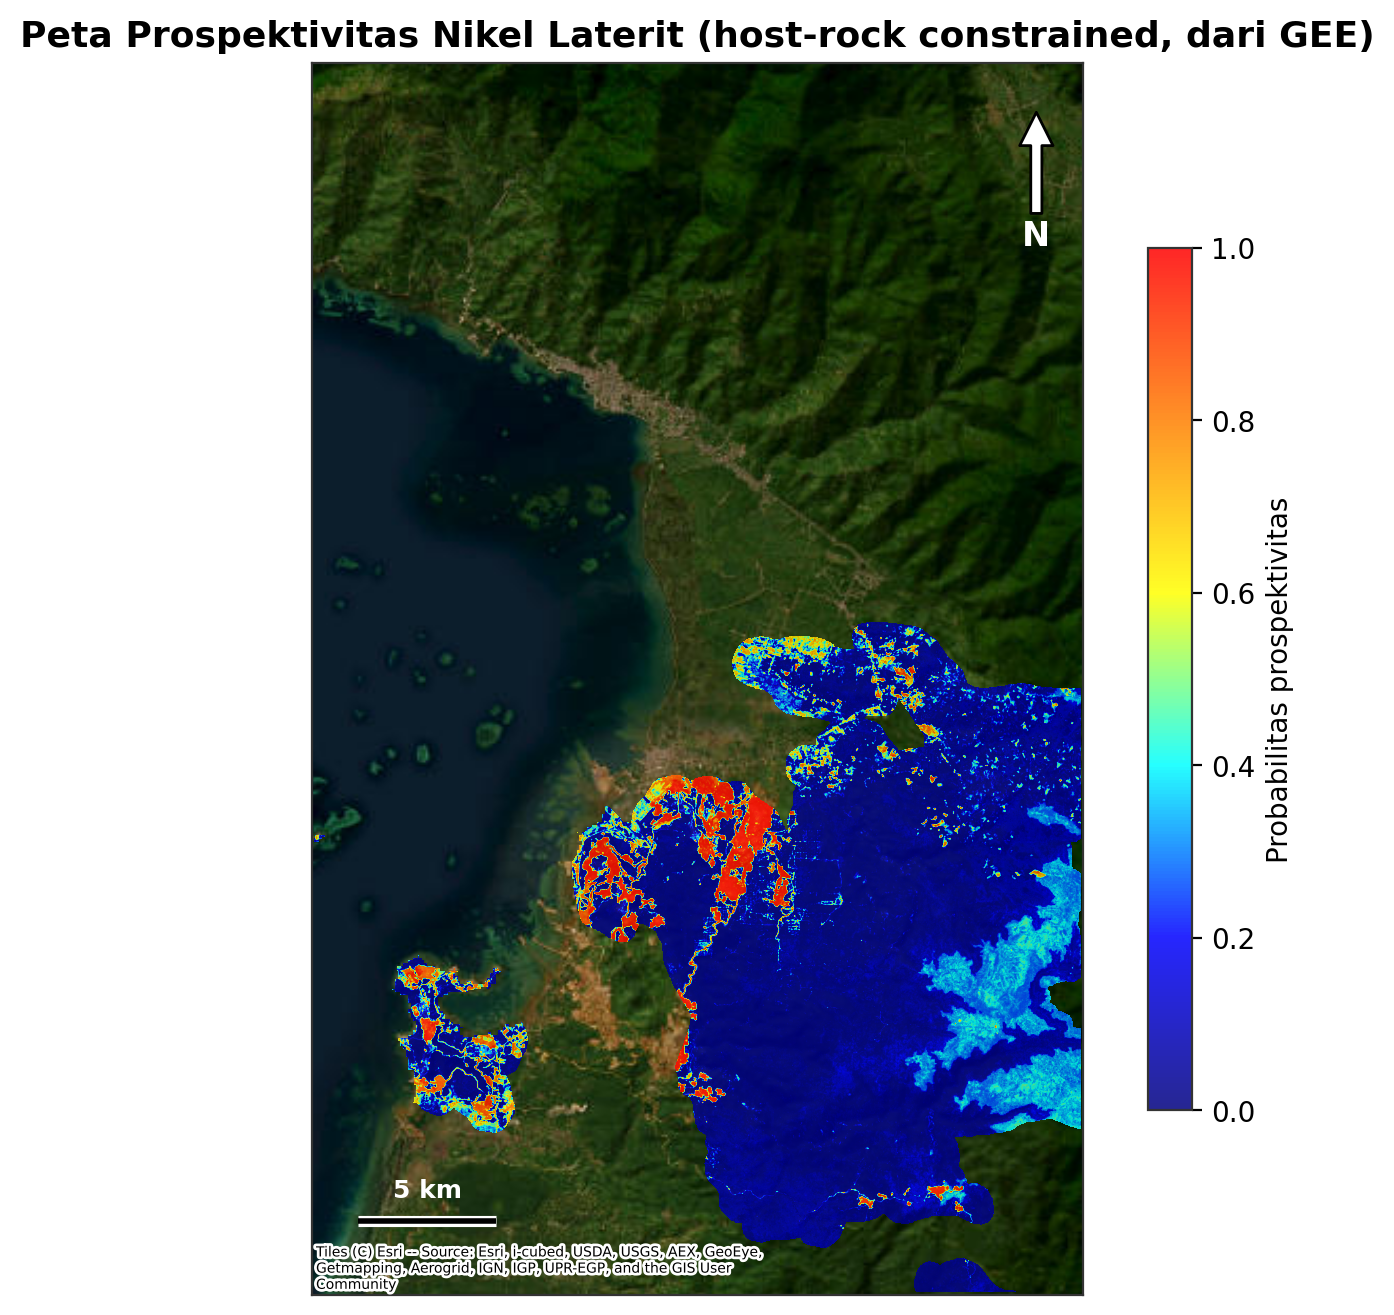
\includegraphics[width=0.86\linewidth]{figures/fig10_prospektivitas.png}
  \caption{Peta prospektivitas nikel laterit final (host-rock constrained).
  Gradasi warna menunjukkan probabilitas keterdapatan; zona merah = prioritas bor.}
  \label{fig:final}
\end{figure}

% ===================================================================
\section{Purwarupa \& Dampak}

\subsection{Target Purwarupa}
WebGIS dashboard interaktif \textbf{NickelScope} (Streamlit + Folium / GEE App):
peta probabilitas, layer \textbf{No-Go ESG}, tabel \textbf{ranking target bor}
(koordinat + skor + keyakinan), dan peta ketidakpastian.

\subsection{Dampak \& Manfaat}
\begin{itemize}
  \item \textbf{Hemat biaya:} fokus bor ke zona high-probability menekan area bor non-produktif.
  \item \textbf{Efisiensi waktu:} mempersempit target sebelum mobilisasi alat berat.
  \item \textbf{ESG \& Safety:} layer no-go \& peta ketidakpastian mengurangi jejak
  lingkungan dan mendukung keputusan sadar-risiko.
  \item \textbf{Reproducible:} 100\% data publik + open-source, mudah diaudit \& dikembangkan.
\end{itemize}

% ===================================================================
\section{Feasibility, Keterbatasan \& Roadmap}

\textbf{Feasibility.} Seluruh data gratis; stack open-source (Python, Google Earth
Engine, scikit-learn, GeoPandas, Streamlit). Pipeline end-to-end sudah berjalan
dan menghasilkan model + peta + 10 figure.

\textbf{Keterbatasan (didokumentasikan jujur).}
\begin{itemize}
  \item Model condong ke fitur spektral $\Rightarrow$ kuat mendeteksi laterit
  \textit{tersingkap}; potensi \textit{di bawah tutupan} perlu penguatan fitur geologi-topografi.
  \item Label berbasis proxy permukaan; validasi lapangan \& data bor nyata akan meningkatkan akurasi.
  \item Buffer host-rock (500 m) dapat dikalibrasi dengan data lapangan.
\end{itemize}

\textbf{Roadmap.}
\begin{enumerate}
  \item Integrasi data bor internal ANTAM (retrain dengan label sebenarnya).
  \item Validasi lapangan \& kalibrasi model.
  \item Varian model ``deteksi'' (spektral) vs ``prospektivitas'' (topografi+geologi).
  \item Ekspansi multi-komoditas \& integrasi ke sistem perencanaan eksplorasi ANTAM.
\end{enumerate}

% ===================================================================
\section{Pemetaan ke Kriteria Penjurian}

\begin{tabularx}{\linewidth}{@{}>{\bfseries}l c Y@{}}
\toprule
Kriteria & Bobot & Bagaimana NickelScope unggul \\
\midrule
Problem \& metodologi   & 25\% & Komoditas prioritas ANTAM; metodologi jujur (spatial CV + host-rock audit) \\
Kreativitas \& teknologi & 25\% & Fusi geospasial + ML + feature engineering geologi + koreksi sirkularitas \\
Kualitas purwarupa      & 25\% & Pipeline berjalan, peta profesional, WebGIS demoable \\
Dampak \& implementasi  & 15\% & De-risking bor + roadmap integrasi ANTAM \\
Presentasi              & 10\% & Narasi kuat ``dari model menyesatkan ke model jujur'' + peta dramatis \\
\bottomrule
\end{tabularx}

\vspace{1em}\hrule\vspace{0.5em}
{\small\color{darkgray}\textit{Repositori \& reproduktibilitas:} seluruh kode
(GEE + Python), data, dan figure tersedia terbuka. Data geologi bersumber dari
Badan Geologi ESDM (GeoMap). Disusun untuk ANTAM Hackathon 2026.}

\end{document}
